\section{Benchmark Design}
\label{sec:method}

\subsection{Design Goals}

DiagBench is a verifier-grounded evaluation framework for engineering design agents, instantiated here on VEH design. The goal is not to create a larger endpoint leaderboard, but to make four load-bearing engineering decisions separately measurable under the same physical oracle. We use four design goals:
\begin{itemize}[leftmargin=5mm,itemsep=1mm,topsep=1mm]
    \item \textbf{Auditable validity:} physical feasibility and objective values must be decided by an external analytical oracle, not by language-model consensus.
    \item \textbf{Stage-specific diagnostics:} each decision boundary should have its own action space, trusted state, and headline metric.
    \item \textbf{Path-dependence visibility:} recovery from corrupted state should remain separate from repair from a clean initial design.
    \item \textbf{Policy visibility:} final selection should test whether the model follows an explicit policy among feasible candidates, not only whether it can generate a design.
\end{itemize}

\begin{figure*}[t]
\centering
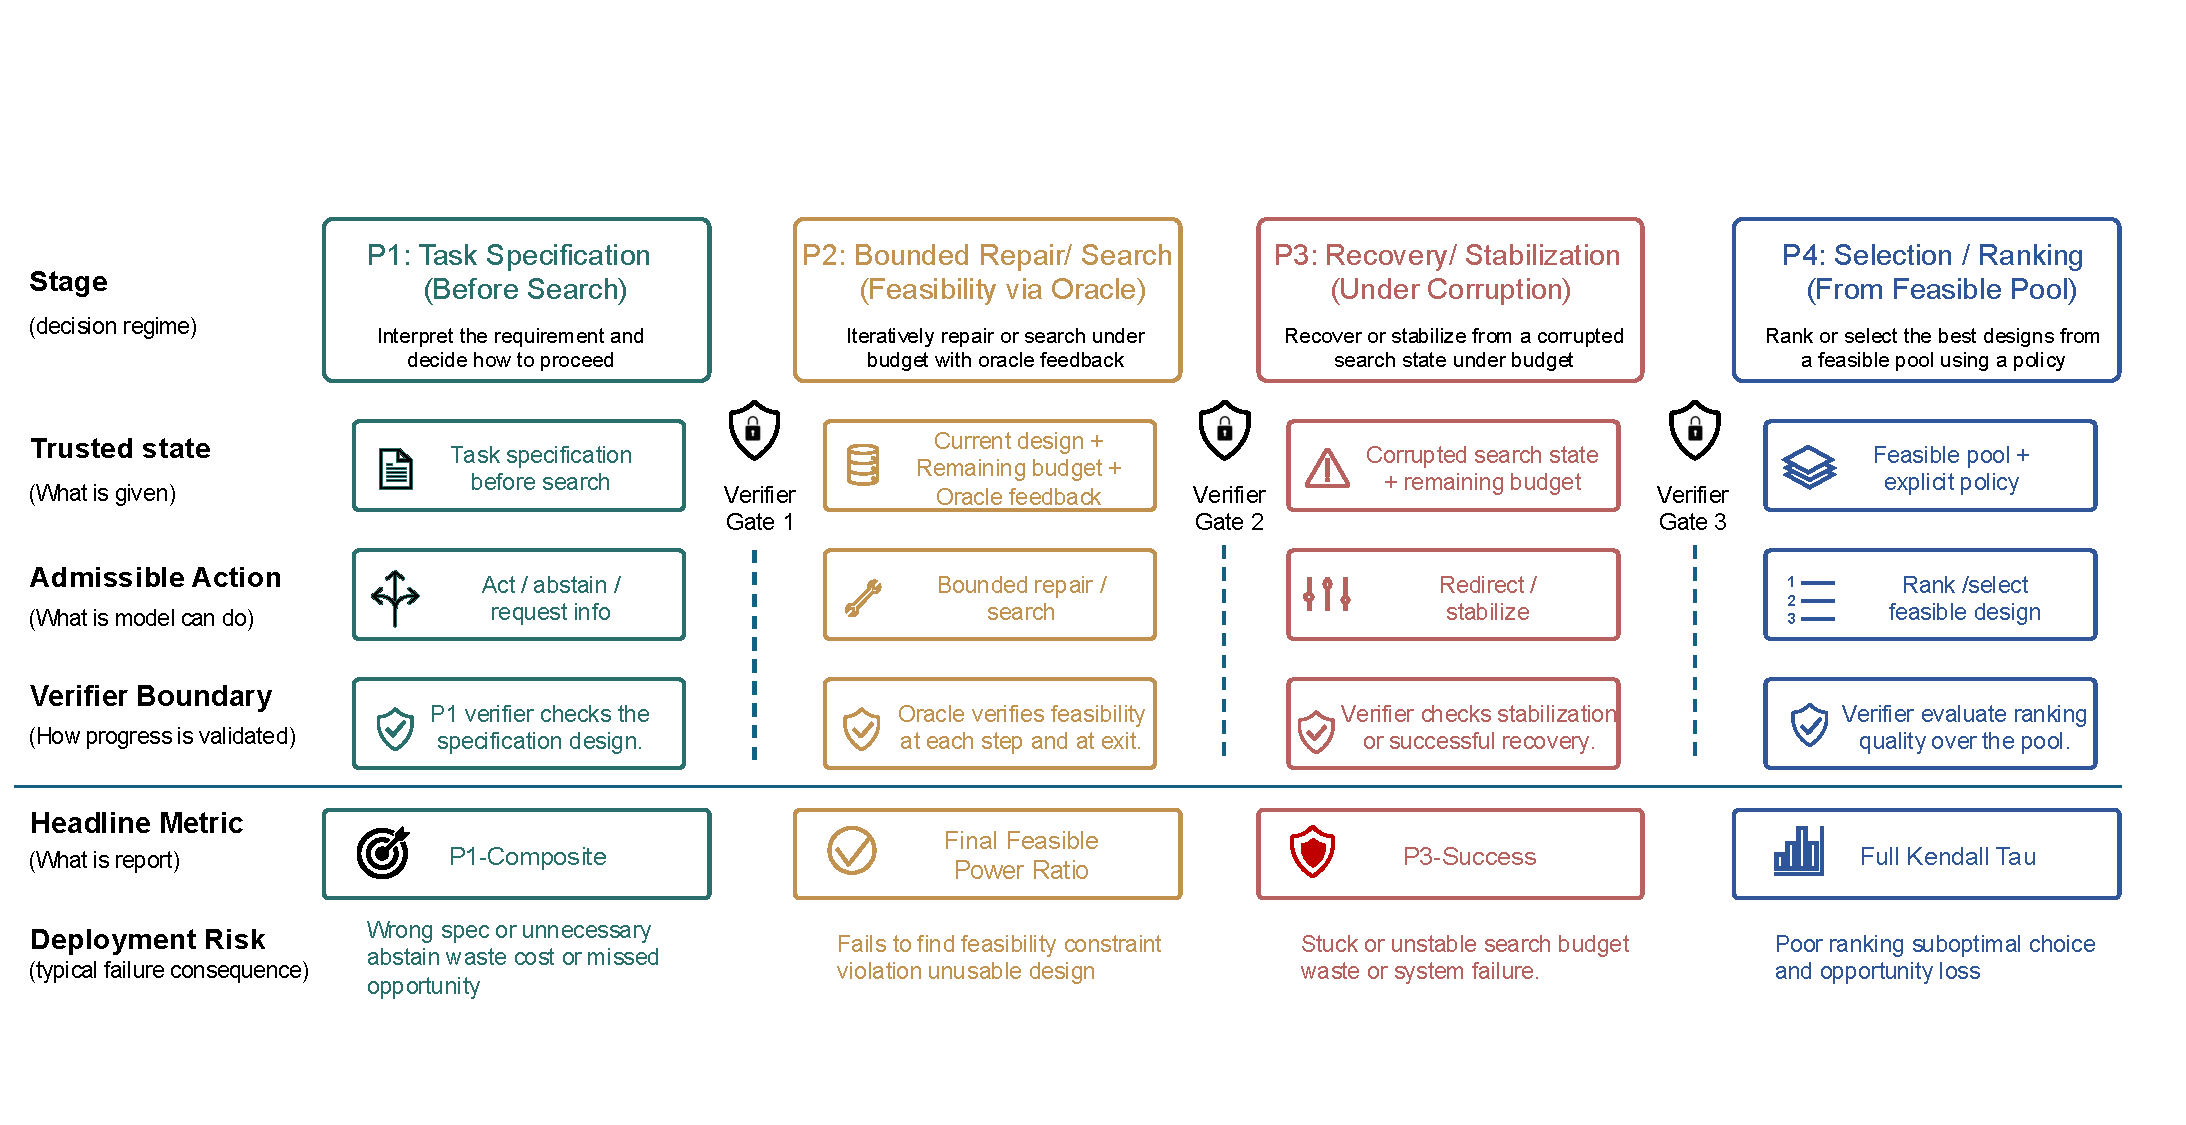
\includegraphics[width=\linewidth]{figures/main/workflow_diagram.pdf}
\caption{DiagBench as a workflow-structured benchmark. Each stage changes the trusted state, the permitted model action, and the headline metric, so endpoint-only evaluation cannot localize which control boundary failed.}
\label{fig:workflow}
\end{figure*}

\textbf{Running example.} A single VEH brief asks for a piezoelectric cantilever resonating at 50 Hz and delivering at least 15\,\textmu W under 0.5\,g excitation. DiagBench turns it into four questions. \textit{P1:} before search, should the agent propose a design, declare infeasibility, or request missing material information? \textit{P2:} from a seed design, can it iteratively repair frequency, power, stress, and displacement violations under oracle feedback? \textit{P3:} after a corrupted history has already moved in a harmful direction, can it reset the trusted state and recover? \textit{P4:} given five oracle-feasible candidates, can it rank them under a declared policy such as ``prioritize output power, then stress margin''? The physical object is shared; the trusted-state boundary is different.

\subsection{Probe Inventory}

\begin{table*}[t]
\caption{DiagBench inventory for the current VEH benchmark. Each probe corresponds to a different workflow boundary and therefore reports a different headline metric.}
\label{tab:inventory}
\centering
\small
\setlength{\tabcolsep}{4pt}
\renewcommand{\arraystretch}{1.08}
\begin{tabular}{lp{30mm}cp{36mm}p{33mm}}
\toprule
Probe & Workflow role & Tasks & Model action & Headline metric \\
\midrule
P1 & Credible triage & 240 & act, abstain, or request information & P1-Composite \\
P2 & Constrained repair/search & 208 & iterative verifier-guided edit & Final feasible power ratio \\
P3 & Post-trap recovery & 156 & reset or stabilize corrupted state & P3-Success \\
P4 & Policy-conditioned ranking & 159 & rank five feasible candidates & Full Kendall Tau \\
\bottomrule
\end{tabular}
\end{table*}

Table~\ref{tab:inventory} gives the main benchmark structure. P1 is a matched certification stress stage: it uses vetted anchor contexts rendered through subtype-balanced templates and is not claimed as a source-disjoint literature holdout. P2--P4 are optimizer-facing stages with DOI-disjoint source-anchor boundaries inherited from the cleaned VEH extraction pipeline. This distinction matters: cross-stage comparisons in this paper are stage-level comparisons under a shared verifier, not claims that all probes instantiate identical split semantics.

\textbf{P1: credible triage.} The model must output exactly one action: \texttt{propose\_design}, \texttt{declare\_infeasible}, or \texttt{request\_missing\_info}. The headline P1-Composite balances macro-F1, acceptance credibility, missing-information discipline, infeasibility discipline, and subtype F1, so raw accuracy alone cannot hide an over-act or over-refuse prior.

\textbf{P2: constrained repair/search.} The model iteratively edits VEH design variables under bounded query budget and oracle feedback. The headline final feasible power ratio rewards both reaching feasibility and preserving utility; first-step feasibility is diagnostic rather than primary.

\textbf{P3: post-trap recovery.} The model starts from a misleading search history that has already moved the design in a harmful direction. P3 separates trap escape, cascade avoidance, and final recovered feasibility; the headline is P3-Success.

\textbf{P4: policy-conditioned ranking.} The model ranks a pool of five oracle-feasible designs under an explicit policy. Full-bank Kendall Tau is the headline, while exact match, top-$k$ agreement, Pareto diagnostics, and BARS audit different ranking failure modes.

\subsection{Construction Pipeline and Oracle Boundary}

\begin{figure*}[t]
\centering
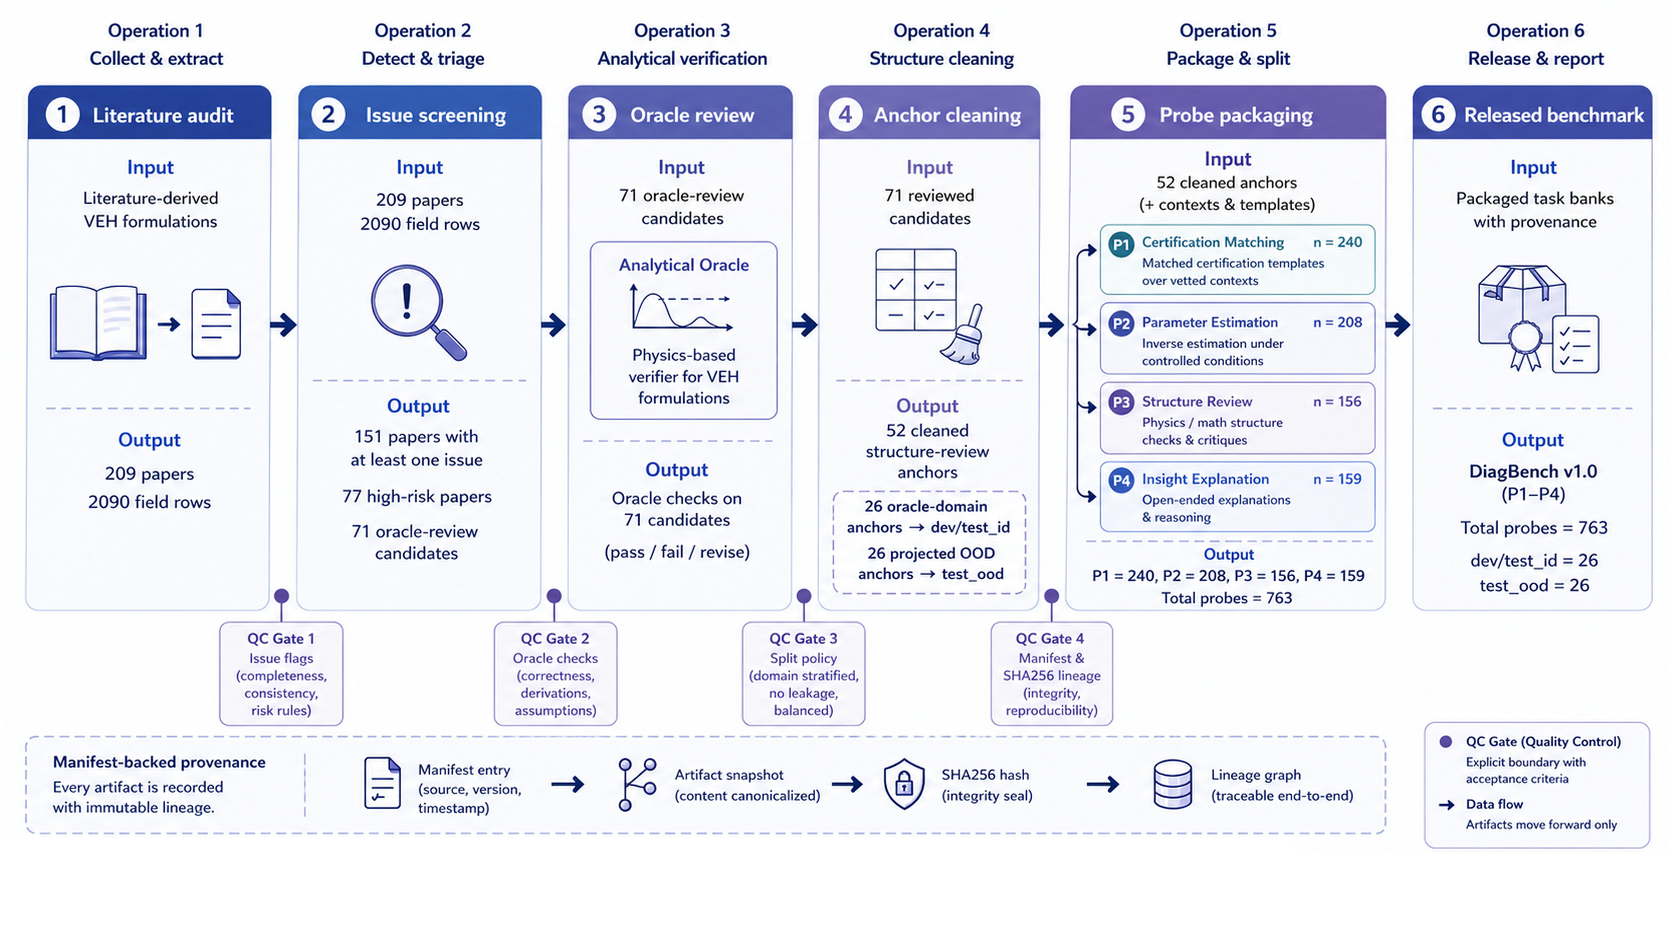
\includegraphics[width=\linewidth]{figures/main/construction_pipeline.pdf}
\caption{Benchmark construction pipeline. The figure summarizes source extraction, verifier review, QC gates, probe packaging, and manifest-backed release.}
\label{fig:construction_pipeline}
\end{figure*}

Figure~\ref{fig:construction_pipeline} summarizes the construction path. The upstream audit covers 209 papers and 2090 extracted field rows, flags high-risk extraction issues, and reduces the corpus to 71 oracle-review cantilever candidates. The current P2 backbone admits 52 cleaned structure-review anchors: 26 oracle-domain anchors routed into DOI-disjoint \texttt{dev}/\texttt{test\_id} splits and 26 projected out-of-domain-kept anchors routed to \texttt{test\_ood}. P3 and P4 inherit this optimizer-facing boundary. Eight unit-suspect papers remain explicitly flagged rather than silently rewritten. Full construction counts, split provenance, and intervention-subset sampling appear in Appendix Tables~\ref{tab:appendix_construction_audit},~\ref{tab:appendix_p3_subset_provenance}, and~\ref{tab:appendix_p3_intervention_delta_ci}.

The oracle boundary is fixed across probes. Each task specifies design variables, bounds, objectives, budgets, and any exposed history. Each proposal is parsed into a JSON action and passed to an analytical verifier, which returns feasibility, active violations, boundary-state labels, and objective information. Physical validity therefore remains external to the model. P2 may stop on feasible closure; P3 preserves the recovery trace so escape, late cascade, and dead-budget behavior remain observable.

The P3 intervention changes only the prompt-facing state representation. In raw-history mode, the model sees the corrupted trajectory. In \texttt{state\_summary} mode, it sees a deterministic verifier-authored summary of trusted fields: latest proposal, active violations, best-so-far feasible design, trend information, and remaining budget. The evaluator, stored trajectory, and oracle are unchanged. This makes the intervention a protocol audit of state isolation rather than a new benchmark variant.

\subsection{Artifact Availability}

The release artifact mirrors the benchmark claims: P1--P4 JSONL task banks, manifests, oracle and evaluator code, generation scripts, admission and split reports, and per-model JSONL logs. Contamination resistance is scoped to DOI/title deduplication, DOI-disjoint source-anchor separation for P2--P4, manifest-level lineage, and no duplicate task ids. We do not claim web-scale pretraining decontamination or model-specific near-duplicate removal. All artifacts are released under CC-BY-4.0 for data and MIT for code, with a Croissant metadata record documenting task schema, split policy, and intended use as an engineering-agent diagnostic benchmark. The benchmark is not intended for production safety certification or as a standalone engineering solver. A frozen anonymous release is available at the URL in the submission; maintenance will follow the DiagBench repository with versioned task banks and per-release manifest hashes.
